\documentclass[border=3pt]{standalone}

%%Fonts
%\usepackage{fontspec}
%\setmainfont[Mapping=tex-text]{Times New Roman}
%\setmonofont[Mapping=tex-text]{JetBrains Mono}

%Drawing
\usepackage{tikz}
\usetikzlibrary{calc, positioning}

% Circuits
\usepackage{circuitikz}

% Lengths
\def\instrdeclen{7}
\def\fsmlen{10}
\def\condlogiclen{4}
\def\width{10.5}

% Node specifics
\def\fillcolor{cyan!60}
\def\innderlabelfont{\scriptsize}

% Connections
\def\outlen{1.5cm}

\tikzset{
every node/.style={rounded corners=0.5cm},
% Instruction Decoder
instr_dec/.style={
	muxdemux,
	muxdemux def={
			Lh=\instrdeclen, Rh=\instrdeclen, w=\width, square pins=1,
			inset Lh=0, inset Rh=0, inset w=0,
			NL=2, NR=5, NB=2, NT=0,
		},
	muxdemux label ={
			L1=op, L2=funct,
			R1=RegSrc, R2=ALUSrc, R3=MemtoReg, R4=ALUControl, R5=ImmSrc,
			B1=NoWrite\_in, B2=BL\_in,
		},
	circuitikz/muxdemuxes/fill=\fillcolor,
	circuitikz/muxdemux/inner label font=\innderlabelfont,
	},
% FSM
fsm/.style={
	muxdemux,
	muxdemux def={
			Lh=\fsmlen, Rh=\fsmlen, w=\width, square pins=1,
			inset Lh=0, inset Rh=0, inset w=0,
			NL=3, NR=7, NB=0, NT=0,
		},
	muxdemux label ={
			L1=op, L2=S/L, L3=R\_d,
			R1=IRWrite, R2=RegWrite, R3=MAWrite, R4=MemWrite, R5=FlagsWrite, R6=PCSrc, R7=PCWrite,
			B1=NoWrite\_in,
		},
	circuitikz/muxdemuxes/fill=\fillcolor,
	circuitikz/muxdemux/inner label font=\innderlabelfont,
	},
% Conditional Logic
cond_logic/.style={
	muxdemux,
	muxdemux def={
			Lh=\condlogiclen, Rh=\condlogiclen, w=\width, square pins=1,
			inset Lh=0, inset Rh=0, inset w=0,
			NL=2, NR=0, NB=0, NT=1,
		},
	muxdemux label ={
			L1=cond, L2=flags,
			T1=CondEx\_in,
		},
	circuitikz/muxdemuxes/fill=\fillcolor,
	circuitikz/muxdemux/inner label font=\innderlabelfont,
	},
% Label
label/.style={
	font=\large\bfseries,
	align=center,
},
% Connection
connection/.style={
	thin,
},
% Input
input/.style={
	font=\scriptsize\ttfamily, above, xshift=-0.2cm,
},
% Output
output/.style={
	font=\ttfamily, right,
},
}

\begin{document}
	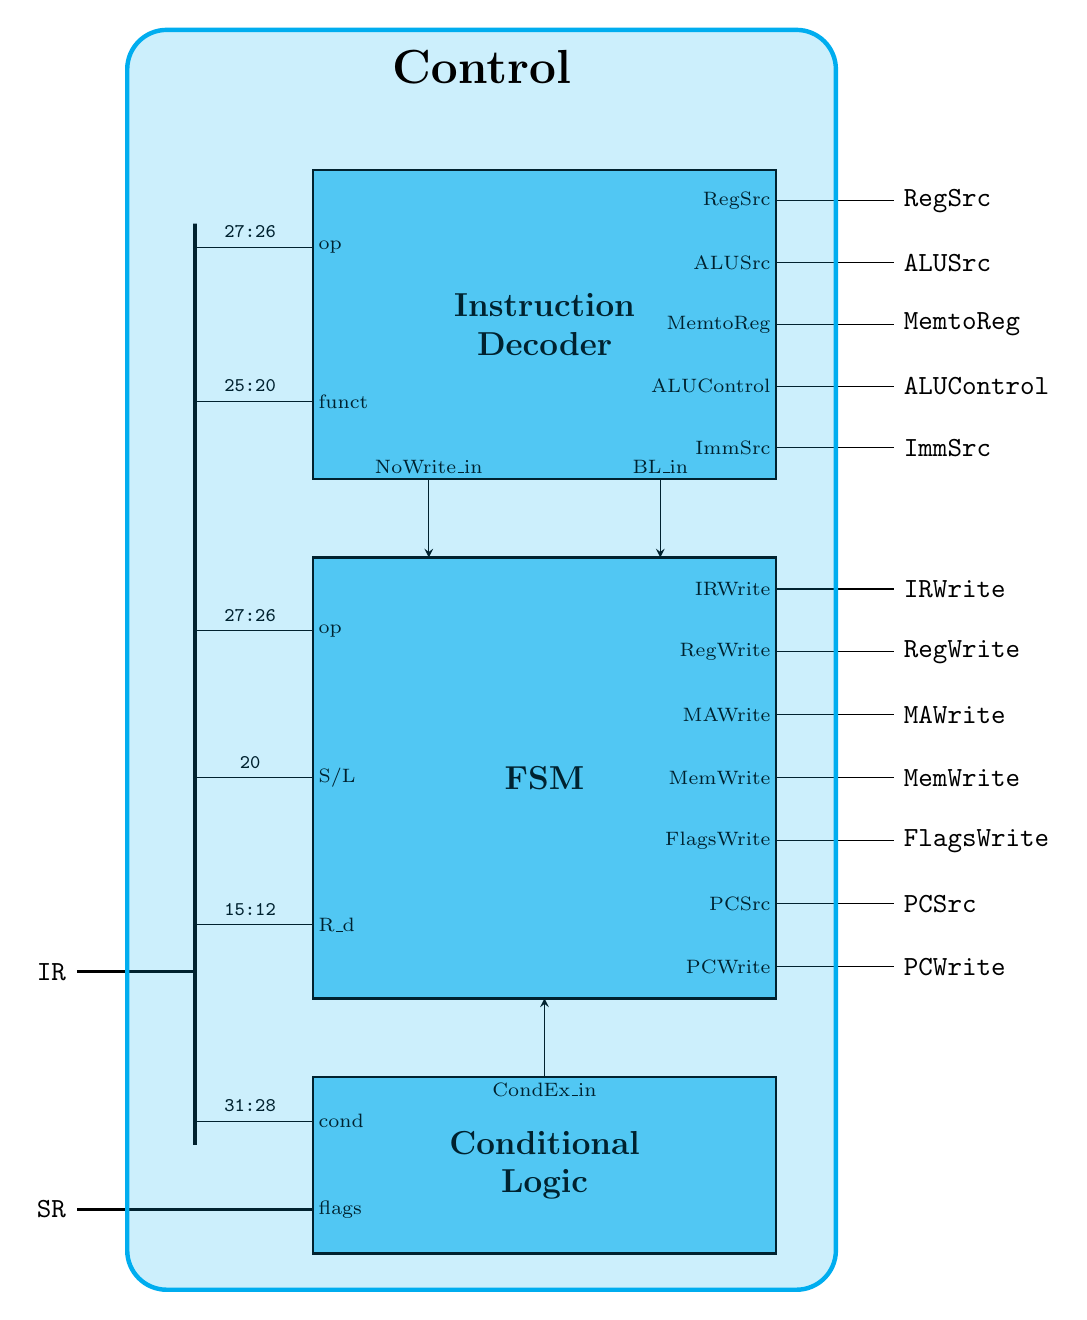
\begin{tikzpicture}[node distance = 1cm]
		% Components
		\node[instr_dec, label] 
			 (instr_dec) {Instruction\\Decoder};

		\node[fsm, label, anchor = north, below=of instr_dec.south] 
			 (fsm) {FSM};

		\node[cond_logic, label, anchor = north, below=of fsm.south] 
			 (cond_logic) {Conditional\\Logic};
			 
			 
		% Connections
		
		% Instruction Decoder Output
		\draw[connection] (instr_dec.brpin 1) -- ++(\outlen,0) node[output] {RegSrc};
		\draw[connection] (instr_dec.brpin 2) -- ++(\outlen,0) node[output] {ALUSrc};
		\draw[connection] (instr_dec.brpin 3) -- ++(\outlen,0) node[output] {MemtoReg};
		\draw[connection] (instr_dec.brpin 4) -- ++(\outlen,0) node[output] {ALUControl};
		\draw[connection] (instr_dec.brpin 5) -- ++(\outlen,0) node[output] {ImmSrc};
		%
		\draw[connection] (instr_dec.blpin 1) -- ++(-\outlen,0) node[input, pos=0.4] {27:26};
		\draw[connection] (instr_dec.blpin 2) -- ++(-\outlen,0) node[input, pos=0.4] {25:20};
		
		% FSM Input
		\draw[connection, -stealth] (cond_logic.top) -- (fsm.bottom); 
		\draw[connection, -stealth] (instr_dec.bbpin 1) -- (instr_dec.bbpin 1|-fsm.top);
		\draw[connection, -stealth] (instr_dec.bbpin 2) -- (instr_dec.bbpin 2|-fsm.top);
		%
		\draw[connection] (fsm.blpin 1) -- ++(-\outlen,0) node[input, pos=0.4] {27:26};
		\draw[connection] (fsm.blpin 2) -- ++(-\outlen,0) node[input, pos=0.4] {20};
		\draw[connection] (fsm.blpin 3) -- ++(-\outlen,0) node[input, pos=0.4] {15:12};
		
		% FSM Output
		\draw[connection] (fsm.brpin 1) -- ++(\outlen,0) node[output] {IRWrite};
		\draw[connection] (fsm.brpin 2) -- ++(\outlen,0) node[output] {RegWrite};
		\draw[connection] (fsm.brpin 3) -- ++(\outlen,0) node[output] {MAWrite};
		\draw[connection] (fsm.brpin 4) -- ++(\outlen,0) node[output] {MemWrite};
		\draw[connection] (fsm.brpin 5) -- ++(\outlen,0) node[output] {FlagsWrite};
		\draw[connection] (fsm.brpin 6) -- ++(\outlen,0) node[output] {PCSrc};
		\draw[connection] (fsm.brpin 7) -- ++(\outlen,0) node[output] {PCWrite};
		
		% Conditional Logic Input
		\draw[connection] (cond_logic.blpin 1) -- ++(-\outlen,0) node[input, pos=0.4] {31:28};
		\draw[connection] (cond_logic.blpin 2) -- ++(-\outlen,0) coordinate (in);
		
		% Input to Control Unit
		\draw[very thick]
			 ($(fsm.left)!0.5!(cond_logic.left) + (-3cm,0)$) node[output, left] (IR) {IR} -- 
			 (IR-|in) -- 
			 ($(in|-instr_dec.lpin 1) + (0,0.3)$) --
			 ($(in|-cond_logic.lpin 1) + (0,-0.3)$);
			 
		\draw[very thick]
			 (cond_logic.blpin 2) -- ++(-3cm,0) node[output, left] {SR};
						   
		\node[
			draw, 
			ultra thick, 
			cyan, 
			fill=cyan,
			fill opacity=0.2,
			rectangle, 
			minimum height=16cm, 
			minimum width=9cm, 
			yshift=1.5cm,
			xshift=-0.8cm] (control) at (fsm) {};
		\node[yshift=-0.5cm] at (control.north) {\LARGE\bfseries Control};
	\end{tikzpicture}
\end{document}



























